\section{Sprint 3}

\subsection{Sprint planning}
	In sprint 3 the group planned on implementing the final requirements with high priority, as well as most of the requirements with medium priority. This is the second to last sprint, and it is important that in the last sprint the  only remaining requirements are medium to low requirements, so that time can also be spent fixing bugs and make the game work properly on iOS. The goal for this sprint will be to get a fully playable game, with only minor requirements missing.

	A usability test will be carried out in the last week of the sprint to discover potential bugs or errors we have yet to discover, as well as ideas for improvements that may be implemented in the next sprint.

	Concerning the report, we plan to finish the content up until this sprint.

\subsection{Duration and workload}
	
	{\bf Duration:} 14.10 - 27.10 (2 weeks)\\
	{\bf Workload:} This is the list with hours spent (the whole grup) on the project in this sprint.
	\begin{itemize}
		\item {\bf Planning:} 15.5 hours
		\item {\bf Development:} 44 hours
		\item {\bf Design:} 0 hours
		\item {\bf Documentation (report):} 59.5 hours
		\item {\bf Testing:} 20.5 hours 
	\end{itemize}
	{\bf Total workload: } 139.5 hours \\
	The group's goal was to work at least 20 hours pr/person every week in this sprint. 
	The group did manage the a workload with an avrage of 17.4 hours/week (139.5 hours/4 persons/2 weeks = 20.6 hours). The reason for the low numbers is because one of the group members did not
	participate as much as he should. The 3 other group members did work over 20 hours. 


\clearpage
\subsection{Sprint backlog}

	\begin{tabular}{| p{1.2cm} | p{8cm} | p{3cm} |}
		\hline
		\rowcolor{gray}
		ID & Description & Estimate \\ \hline

		FR2.5 & The amount of power available to the user should be limited; 
		the power supply of a power plant should be upgradeable. & \\ \hline

		FR2.6 & The user should be able to remove power lines from the 
		& \\ \hline

		FR2.7 & The player should only be allowed to build a level-specific 
		number of power plants. & \\ \hline

		FR3.1 & Arbitrary power lines may be damaged throughout the game & \\ \hline

		FR3.2 & The user should be able to fix unstable power lines before it is 
		broken; this should cost some amount of money. & \\ \hline

		FR3.3 & There should be several types of buildings on the map, with different 
		power requirements & \\ \hline

		FR3.4 & Different types of building should reward different amounts of 
		money & \\ \hline

		FR4.1 & The user should be able to continue to the next level when the goal is 
		reached & \\ \hline

		FR4.3 & As the user reaches higher levels new buildings appear more 
		rapidly & \\ \hline

		FR4.4 & As the user reaches higher levels unstable power lines will appear 
		more rapidly & \\ \hline

		FR4.5 & As the user reaches higher levels the map size may increase & \\ \hline

		FR4.6 & The user should be able to win the game by reaching the goal in 
		the current level. The goal is level specific. & \\ \hline

		FR5.2 & When connecting buildings through power cables, there should be a 
		cost which is proportional to the length of the cable. & \\ \hline

		FR6.11 & The user should be able to see which houses is selected when 
		building power cables & \\ \hline

		FR6.12 & The cables should change color if it is connected to a power 
		station. & \\ \hline

		FR6.13 & The user should be able to see how much power the powerplant have 
		left. This bar should decrease if a building is connected to the powerplant 
		and should be increase if a building is removed. The colors should be yellow 
		with white background. & \\ \hline

	\end{tabular}

\subsection{Implementation}

	Write about algorithms and implementations done!
	
	\begin{figure}[H]
		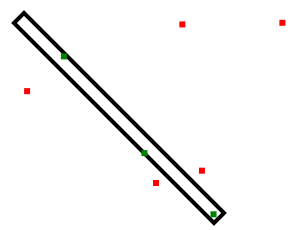
\includegraphics[scale=0.6]{pictures/touchInStroke.png}
		\caption{Test code running}
	\end{figure}

\subsection{Testing}

	\definecolor{lightgray}{gray}{0.9}

	\begin{tabular}{| p{2cm} | p{7cm} | p{3cm} |}
		\hline
		\rowcolor{lightgray}
		{\bf Test Case} & {\bf Result} & {\bf Pass/Not pass} \\ \hline

	  	FT-06 Build Power Lines &  &  \\ \hline

	  	FT-11 Collect Money &  &  \\ \hline

	  	FT-14 Win Game &  &  \\ \hline
	  	
	  	FT-16 Limited Power &  &  \\ \hline
	  	
	  	FT-17 Remove Power Cables &  &  \\ \hline
	  	
	  	FT-18 Number of Power Plants &  &  \\ \hline
	  	
	  	FT-19 Different Buildings &  &  \\ \hline

	  	FT-20 Damaged Power Lines &  &  \\ \hline
	  	
	  	FT-21 Enter next level &  &  \\ \hline

	  	FT-22 Appearance of buildings in new levels &  &  \\ \hline

	  	FT-23 More unstable power lines in new levels &  &  \\ \hline

	  	FT-25 Selected houses &  &  \\ \hline

	  	FT-26 Color of power cable &  &  \\ \hline

	\end{tabular}

\subsection{Changes to the requirements}

	As we worked during thi sprint we made some changes to the requirement specification.
	The first is FR 1.2 that we changed priority on. 

	The requirement (FR 6.5) with notification for new obstacles is removed. 
	The group defined a sound as a notification and will discuss within the group if
	we want to have a sound of not, but the visual notification will not be implemented. 

	Since the game is in a state where it is playable we have focused some more on the 
	GUI, and therefore have added some new requirements (FR 1.11 - FR 1.13) that were missing 
	from the specification.
	
	{\bf All changes on version 3 of the requirement specification:} \\
	\begin{tabular}{| p{1.5cm} | p{12cm} |}
		\hline
		\rowcolor{lightgray}
		{\bf FR} & {\bf Change} \\ \hline
		FR 1.2 & {\bf \color{orange}[CHANGED PRIORITY FROM HIGH TO MEDIUM]} The user should be able 
		to exit the game at any time, and the game state should be saved and loaded when the user 
		returns to the game \\ \hline
		FR 4.6 & {\bf \color{green}[NEW]} The user should be able to win the game by reaching the goal in the current level. The goal is level specific. \\ \hline
		FR 6.5 & {\bf \color{red}[REMOVED]} The user shoud get a notification of new events outside 
		the screen \\ \hline
		FR 6.11 & {\bf \color{green}[NEW]} The user should be able to see which houses is selected when building power cables. \\ \hline
		FR 6.12 & {\bf \color{green}[NEW]} The cables should change color if it is connected to a power 
		station. \\ \hline
		FR 6.13 & {\bf \color{green}[NEW]} The user should be able to see how much power the 
		powerplant have left. This bar should decrease if a building is connected to the powerplant 
		and should be increase if a building is removed. The colors should be yellow whit white 
		background. \\ \hline
	\end{tabular}


\subsection{Group dynamics}
	As a group, it is important to have fun. In the start of the project, the group had some
	problems with the communication, but this is not a problem anymore.
	When the group work we talk about what we read on reddit, what we did yesterday and 
	"bully" each other for funny writing typo, if found, in this report. 

	The harmony in the group is now great and it helps us keep up the good work and meet 
	our sprint goals. We belive having fun is the key to succeed in this project. 

\subsection{Customer feedback}

\subsection{Sprint retrospective}
	In this sprint, we did not do the sprint retrospective, but all the team members did
	get the chance to add changes to the next and last sprint. We are quite pleased with the way 
	we work and non of the group members had anything specific to add or remove in the next sprint.

	We have only had one situation where two of the team members worked on the same implementation, 
	but we dont think that would happend again and have not been a problem up until now. 
	The group need to ensure a good communication within the group as well as give good status
	updates while working. 

	The group agreed to keep up the good work. "Team spirit!".